\documentclass[12pt,a4letter]{article}
\usepackage{amsmath,amsxtra,amssymb,latexsym, amscd,amsthm}
\usepackage{indentfirst}
\usepackage[mathscr]{eucal}
\usepackage{graphicx}
%\usepackage{txfonts}
\usepackage{picinpar}
%\usepackage{floatflt}
\usepackage[utf8]{vietnam}
\usepackage{epic}
\usepackage{makeidx}
\usepackage{longtable}%
\usepackage{multicol}%
%\voffset=-0.8in
% \hoffset=-2cm
\voffset=-2cm
\textheight 24truecm 
\textwidth 16truecm 
\setlength{\baselineskip}{16truept}
\usepackage{mathpazo}
\usepackage{answers}%[nosolutionfiles]
\newtheorem{btbt}{Câu}%[btdb]
\newenvironment{cauhoi}{\begin{btbt}\rm }{\end{btbt}}
\Newassociation{traloi}{Soln}{goiytraloi}
\renewcommand{\Solnlabel}[1]{{\bf Lời giải #1}.}
\def\tentruong{\small ĐH KHOA HỌC TỰ NHIÊN HÀ NỘI}
\def\tenkhoa{Khoa Toán - Cơ -Tin học}
\def\loaidethi{\textbf{Đề số 1}}%{ĐỀ THI LẠI}%%{ĐỀ CHÍNH THỨC}
\def\tenkythi{ĐỀ THI  HỌC KÌ 2017-2018}
\def\tenmonhoc{Môn thi: Lý thuyết tối ưu}
\def\thoigian{Thời gian làm bài: 90 phút}
\usepackage{centerpage}
\usepackage{systeme}
\sysdelim.. \syseqsep{:}
\graphicspath{{hinh/}}
\begin{document}
\Opensolutionfile{goiytraloi}[traloi] 
\Writetofile{goiytraloi}{\protect\centerline{\bf LỜI GIẢI: \tenkythi -SỐ 1}}

\thispagestyle{empty}
\begin{minipage}[b]{0.45\textwidth}
\centering
{ \tentruong}\\
\tenkhoa\\ %\makebox[4cm]{\hrulefill}\\
\loaidethi\\
\quad \\
%{({\it Đề thi \@scau{} câu / \@strang{} trang})}
\end{minipage}
\hfill
\begin{minipage}[b]{0.5\textwidth}
\centering
{\bf \tenkythi}\\
{\bf  \tenmonhoc}\\
{\it \thoigian}\\
\qquad %{\it \@scau}
\end{minipage}

% ======================================================================================

\vspace*{1cm}

\begin{cauhoi}%1
(3 điểm)
Tìm các phương án cực biên không suy biến của bài toán qui hoạch tuyến tính với các ràng buộc sau:
$$f(x)=x_1+2x_2+4x_3\rightarrow\min$$
$$\begin{cases}
\systeme{
3x_1  -2x_2  +  3x_3  =  6,:
-x_1  +  2x_2  -x_3  =  4,}\\
x_j \ge 0, j = 1, 2, 3.
\end{cases}$$

%%%%%%%%%%%%%%%%%%%Lời giải
\begin{traloi}
Bài toán này có $m = 2$ ràng buộc chính và $n = 3$ biến. Một phương án cực biên có nhiều nhất $m = 2$ thành phần dương, tức là có ít nhất $n - m = 1$ thành phần bằng $0$.
 Vì thế, lần lượt cho $x_1, x_2, x_3$ bằng $0$ ta được:


 Với $x_1 = 0$, hệ phương trình trên cho ta $x_2 = \dfrac{9}{2}; x_3 = 5$.  

 Với $x_2 = 0$, hệ phương trình trên vô nghiệm.

Với $x_3 = 0$, hệ phương trình trên cho ta $x_1 = 5; x_2 =\dfrac{9}{2}.$

 Ta nhận được hai phương án: $\left(0, \dfrac{9}{2}, 5\right)^T$ và $\left(5, \dfrac{9}{2}, 0\right)^T$. 

Kiểm tra trực tiếp cho thấy hệ 2 véctơ $A^2 = (-2, 2)^T, $\break
 $A^3 = (3, -1)^T$ và 
$A^1 = (3, -1)^T, A^2 = (-2, 2)^T$ là độc lập tuyến tính.

Nên cả hai phương án trên đều là các phương án cực biên không suy biến (số thành phần dương bằng $m = 2$).
\end{traloi}
\end{cauhoi}

\begin{cauhoi}%2
(3 điểm)  Giải bài toán quy hoạch tuyến tính sau bằng hình học:
\begin{center}
$f(x,y)=20x+40y\rightarrow\max$\\
$\begin{cases}
\systeme{
6x+y\ge 18,:
x+4y\ge 12,:
2x+y\ge 10,}\\
x,y\ge 0.
\end{cases} $
\end{center}

%%%%%%%%%%%%%%%%%%%Lời giải
\begin{traloi}
Giải bằng phương pháp hình học. Miền các phương án được xác định bằng đa giác lồi mở
$xABCDy$ với $A(12,0), B(4,2), C(2,6), D(0,18)$. Biểu diễn vectơ pháp tuyến $\vec{n}=(1,2)$ và hàm mục tiêu $L(x,y)=20x+40y$ như hình vẽ.

\begin{figure}[!ht]
\centering
%\input hinh24.tex
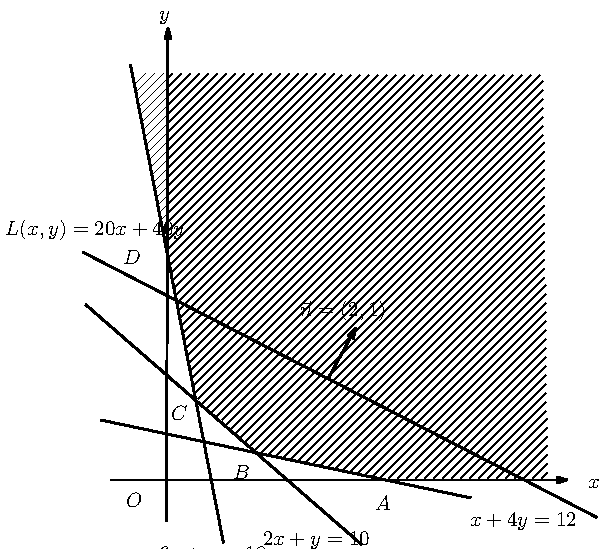
\includegraphics[scale =0.7]{hinh24}
\caption{}\label{fig:2}
\end{figure}

Di chuyển đường hàm mục tiêu ngược với $\vec{n}$ tới vị trí giới hạn là điểm $B(4,2)$. Vậy bài toán không có phương án tối ưu.

\end{traloi}
\end{cauhoi}

\begin{cauhoi}%3
(4 điểm)
Xét bài toán quy hoạch tuyến tính sau đây
$$ f(x)=5x_1+4x_2+6x_3\rightarrow \min$$
\begin{equation*}
\left\{
\begin{array}{r r r l }
2x_1&+4x_2&+3x_3&\ge 48 \\ 
3x_1&+2x_2&+3x_3&\ge 30 \\ 
x_1&+3x_2&+4x_3&\ge 23 \\ 
\multicolumn{4}{l}{x_j\ge 0,\quad j = 1, 2, 3.}\\
\end{array}
\right.
\end{equation*}

a) Hãy đưa bài toán về dạng chính tắc.

b) Giải bài toán bằng phương pháp đơn hình.

%%%%%%%%%%%%%%%%%%%Lời giải
\begin{traloi}
a) Đưa bài toán về dạng chính tắc
$$ f=5x_1+4x_2+6x_3\rightarrow \min$$
\begin{equation*}
\left\{
\begin{array}{r r r r r  r l }
2x_1&+4x_2&+3x_3&-x_4&&&= 48 \\ 
3x_1&+2x_2&+3x_3&&-x_5&&= 30 \\ 
x_1&+3x_2&+4x_3&&&-x_6&= 23 \\ 
\multicolumn{6}{l}{x_j\ge 0,\quad j = 1, 2, 3, 4, 5, 6.}\\
\end{array}
\right.
\end{equation*}
b) Ta biến đổi để xuất hiện biến cơ bản như sau:  Giữ nguyên phương trình thứ nhất, đem nó trừ đi lần lượt các phương trình thứ 2 và 3 cho kết quả mới. Ta có bài toán tương đương
$$ f=5x_1+4x_2+6x_3\rightarrow \min$$
\begin{equation*}
\left\{
\begin{array}{r r r r r  r l }
2x_1&+4x_2&+3x_3&-x_4&&&= 48 \\ 
-x_1&+2x_2&&-x_4&+x_5&&= 18 \\ 
x_1&+x_2&-x_3&-x_4&&+x_6&= 25 \\ 
\multicolumn{6}{l}{x_j\ge 0,\quad j = 1, 2, 3, 4, 5, 6.}\\
\end{array}
\right.
\end{equation*}
Ta đưa về bài toán mở rộng
$$ f=5x_1+4x_2+6x_3\qquad +Mx_7\rightarrow \min$$
\begin{equation*}
\left\{
\begin{array}{r r r r r  r r l }
2x_1&+4x_2&+3x_3&-x_4&&&+x_7&= 48 \\ 
-x_1&+2x_2&&-x_4&+x_5&&&= 18 \\ 
x_1&+x_2&-x_3&-x_4&&+x_6&&= 25 \\ 
\multicolumn{6}{l}{x_j\ge 0,\quad j = 1, 2, 3, 4, 5, 6,7.}\\
\end{array}
\right.
\end{equation*}
Trong đó $x_7$ là biến giả, $M>0$ rất lớn.

\begin{tabular}{| l | l | l | l  l  l  l  l  l  l |}
\hline
$x_B$&$c_B$&PA&$x_1$&$x_2$&$x_3$&$x_4$&$x_5$&$x_6$&$x_7$\\ 
&&&5&4&6&0&0&0&M\\ 
\hline
$x_7$&M&48&[2]&4&3&-1&0&0&1\\ 
$x_5$&0&18&-1&2&0&-1&1&0&0\\ 
$x_6$&0&25&1&1&-1&-1&0&1&0\\
\hline 
f &M&48&2&4&3&-1&0&0&0\\ 
\cline{2-10}
&&0&-5&-4&-6&0&0&0&0\\ 
\hline
$x_1$&5&24&1&2&3/2&-1/2&0&0&\\ 
$x_5$&0&42&0&[4]&3/2&-3/2&1&0&\\ 
$x_6$&0&1&0&-1&-5/2&-1/2&0&1&\\ 
\hline
f&&120&0&6&3/2&-5/2&0&0&\\ 
\hline
$x_1$&5&3&1&0&3/4&1/4&-1/2&0&\\ 
$x_2$&4&21/2&0&1&3/8&-3/8&1/4&0&\\ 
$x_6$&0&23/2&0&0&-17/8&-7/8&1/4&1&\\ 
\hline
f&&57&0&0&-3/4&-1/4&-3/2&0&\\ 
\hline
\end{tabular}

Bài toán đã cho có phương án tối ưu duy nhất là
$x^*=(3, 21/2, 0)^T$ và $f_{\min}=57$.
\end{traloi}
\end{cauhoi}

% \begin{cauhoi}%3
% Cho số liệu bài toán vận tải và ma trận $(c_{ij})$ như sau:
% 
% $(a_i)=(100, 80, 20)^t$ \qquad $(b_j)=(60, 70, 40, 30)$
% 
% $(c_{ij})=\begin{bmatrix}
% 2&1&4&3\\ 
% 5&3&2&6\\ 
% 6&2&1&5\\ 
% \end{bmatrix}$ 
% 
% a) Viết lại nội dung bài toán vận tải trên như bài toán quy hoạch tuyến tính.
% 
% b) Lập bảng vận tải cho bài toán trên.
% 
% c) Tìm phương án xuất phát theo phương pháp cực tiểu cước phí.
% 
% d) Giải bài toán vận tải trên theo phương pháp quy 0 cước phí các ô chọn.
% \begin{traloi}
% a) b) c) như trong sách.
% 
% d) Kết quả nghiệm
% 
% $x^*=\begin{bmatrix}
% 60&10&0&30\\ 
% 0&60&20&0\\ 
% 0&0&20&0\\ 
% \end{bmatrix}$ 
% ,\quad $f(x^*)=460.$
% \end{traloi}
% \end{cauhoi}
% 
% \vspace*{1cm}
% {\bf Chú ý:} Sinh viên không được mang sách giáo trình và vở ghi chép vào phòng thi.
\Closesolutionfile{goiytraloi}
\newpage
\Readsolutionfile{goiytraloi}

\end{document}